\section{Einpuls-Gleichrichter (M1U)}
Bezeichnung Gleichrichter:
\begin{center}
    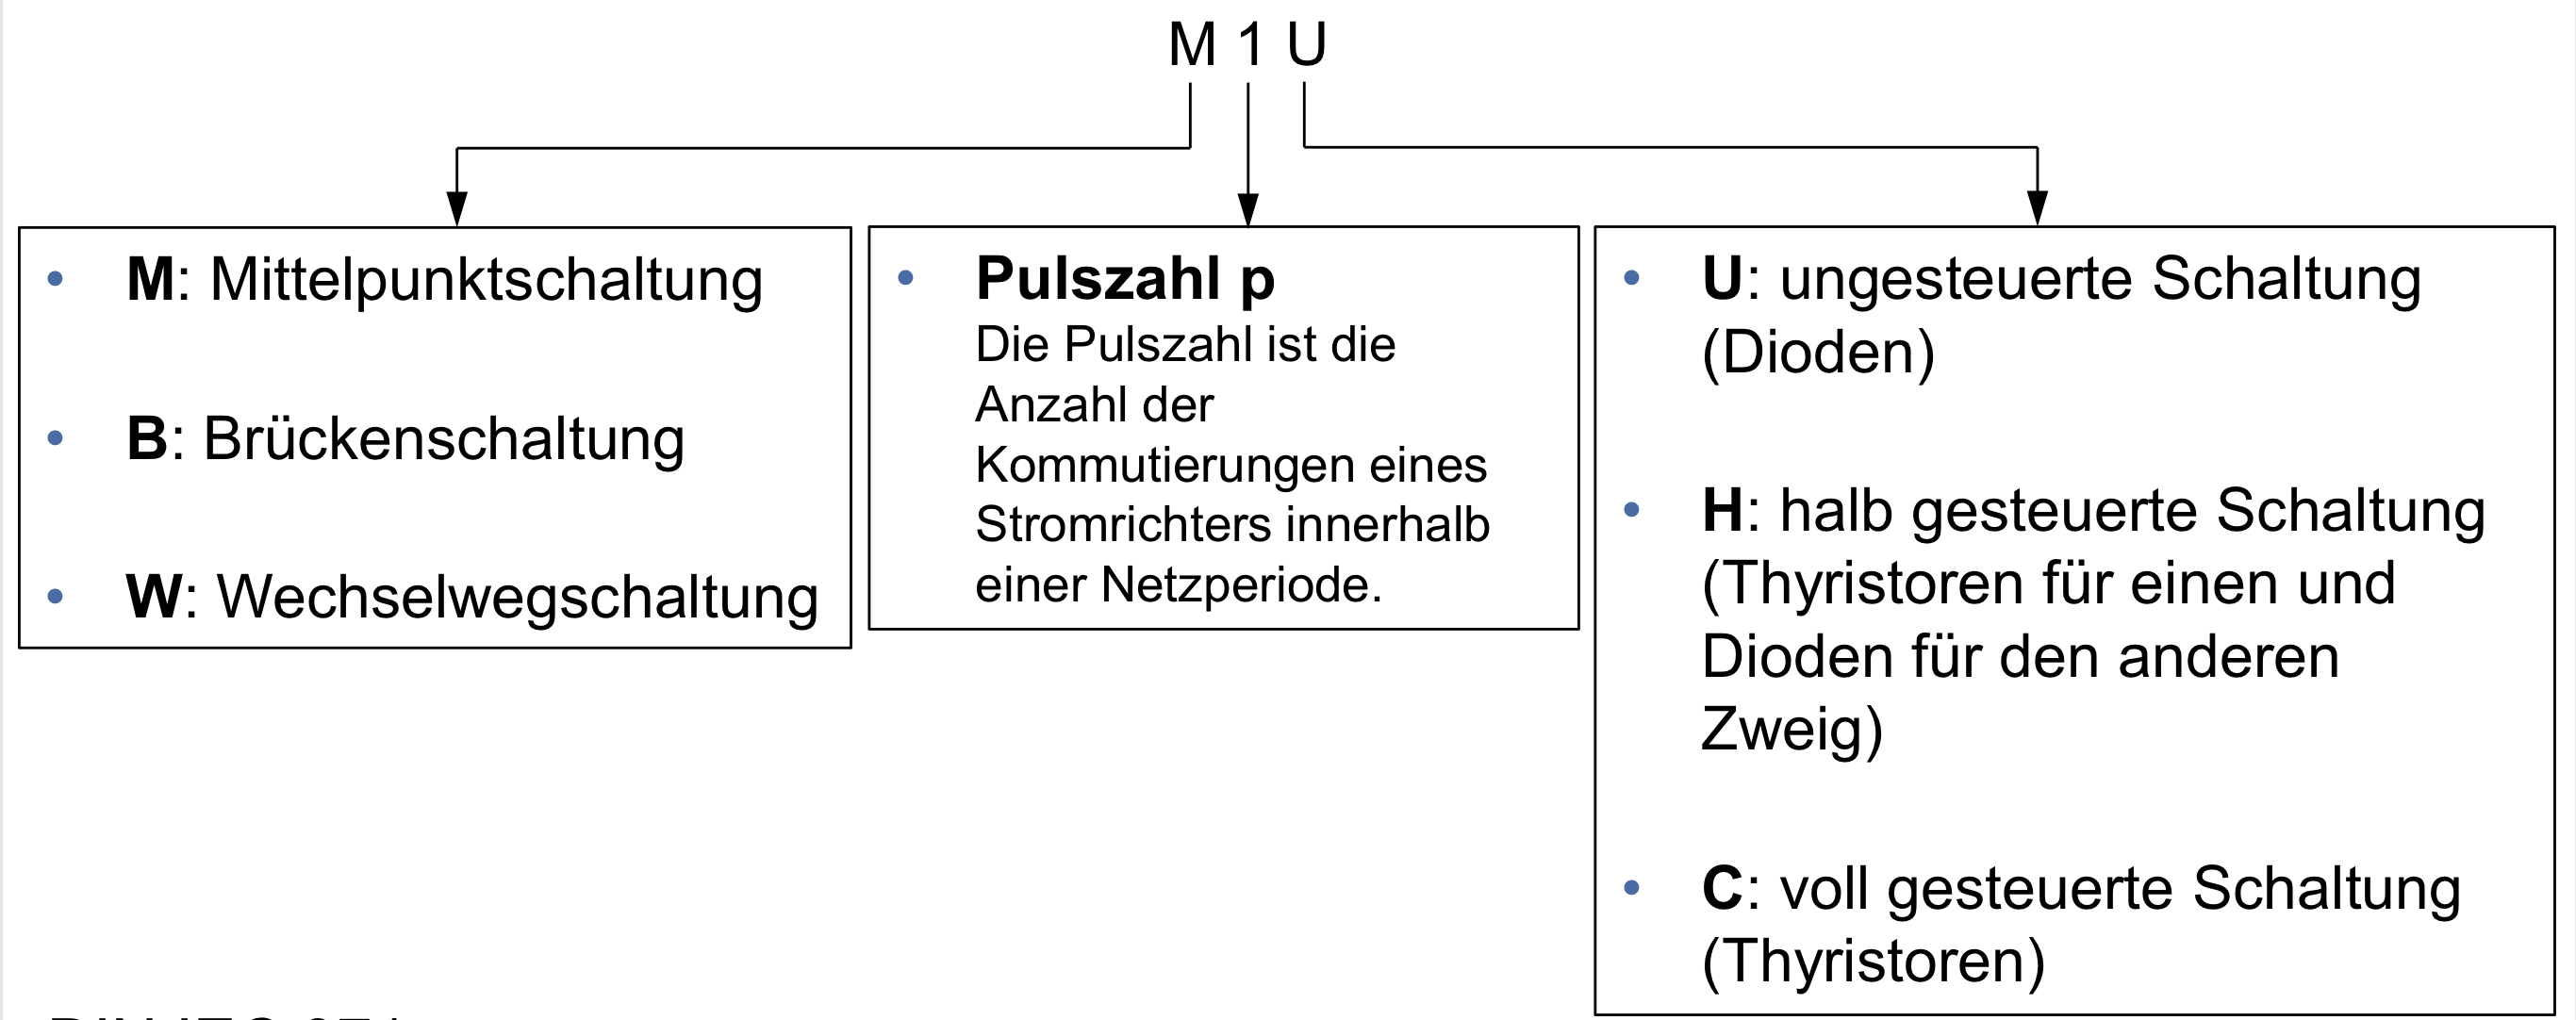
\includegraphics[width=0.85\linewidth]{images/gleichrichterkenn.png}
\end{center}

Diese Section behandelt den \textbf{Einpuls-Gleichrichter (M1U)} als einfachste Gleichrichterschaltung.
Er ist ein zentrales Prüfungs- und Übungsthema zur Berechnung von \textbf{Mittelwert}, \textbf{Effektivwert} und \textbf{Laststrom}
bei ohmscher und induktiver Last.

\smallskip

\textbf{Zielbild:}
\begin{itemize}
    \item Topologie und Funktionsprinzip verstehen
    \item Zeitverlauf der Ausgangsspannung bestimmen
    \item Mittelwert und Effektivwert berechnen
    \item Einfluss der Last (R, R-L) analysieren
\end{itemize}

\subsection{Grundschaltung des Einpuls-Gleichrichters}
\begin{center}
    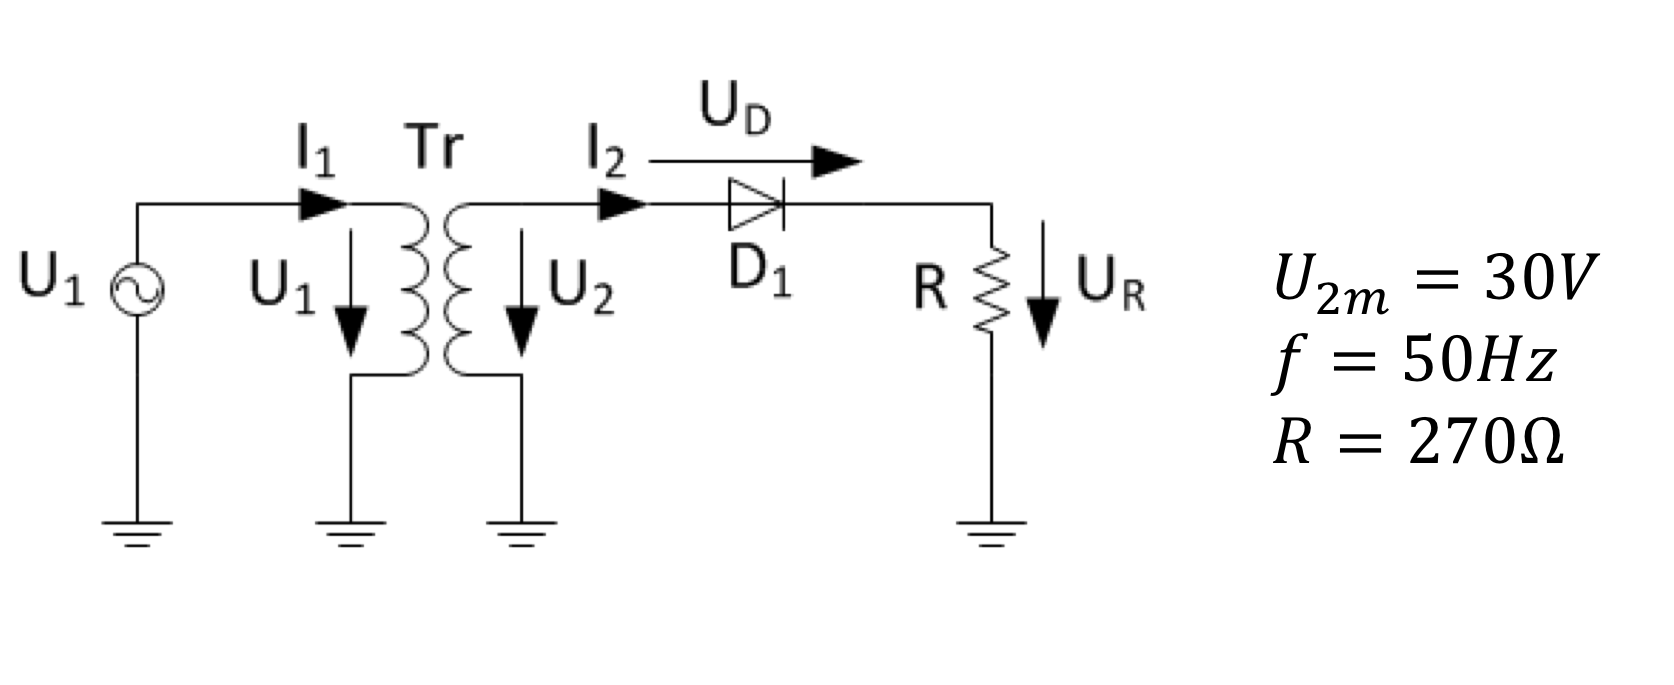
\includegraphics[width=0.85\linewidth]{images/M1U.png}
\end{center}
\begin{center}
    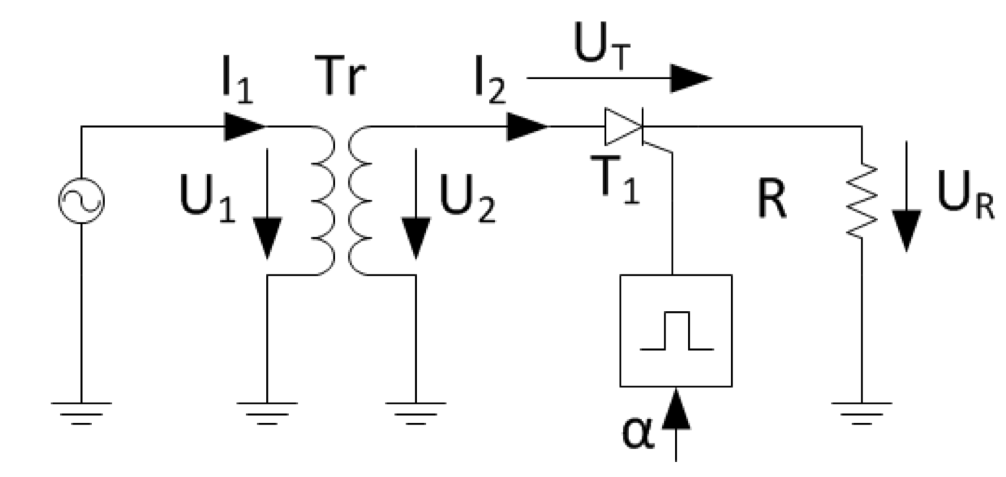
\includegraphics[width=0.85\linewidth]{images/M1C.png}
\end{center}

\textbf{Elemente:}
\begin{itemize}
    \item $u_1(t) = \hat U \sin(\omega t)$: sinusförmige Eingangsspannung
    \item $D$: ideale Diode
    \item $R$ bzw. $R$-$L$: Last
    \item $u_2(t)$: gleichgerichtete Ausgangsspannung
\end{itemize}

\subsection{Funktionsprinzip}

\begin{itemize}
    \item Für $u_1(t) > 0$ leitet die Diode: $u_2(t) = u_1(t)$.
    \item Für $u_1(t) < 0$ sperrt die Diode: $u_2(t) = 0$.
\end{itemize}

Mathematisch:
\[
u_2(t) =
\begin{cases}
\hat U \sin(\omega t), & 0 < \omega t < \pi,\\
0, & \pi < \omega t < 2\pi.
\end{cases}
\]

\crd{\textrightarrow\ Nur die \textbf{positive Halbwelle} trägt zur Ausgangsspannung bei.}

\subsection{Skizze 1: Eingang und Ausgangsspannung}
\begin{center}
    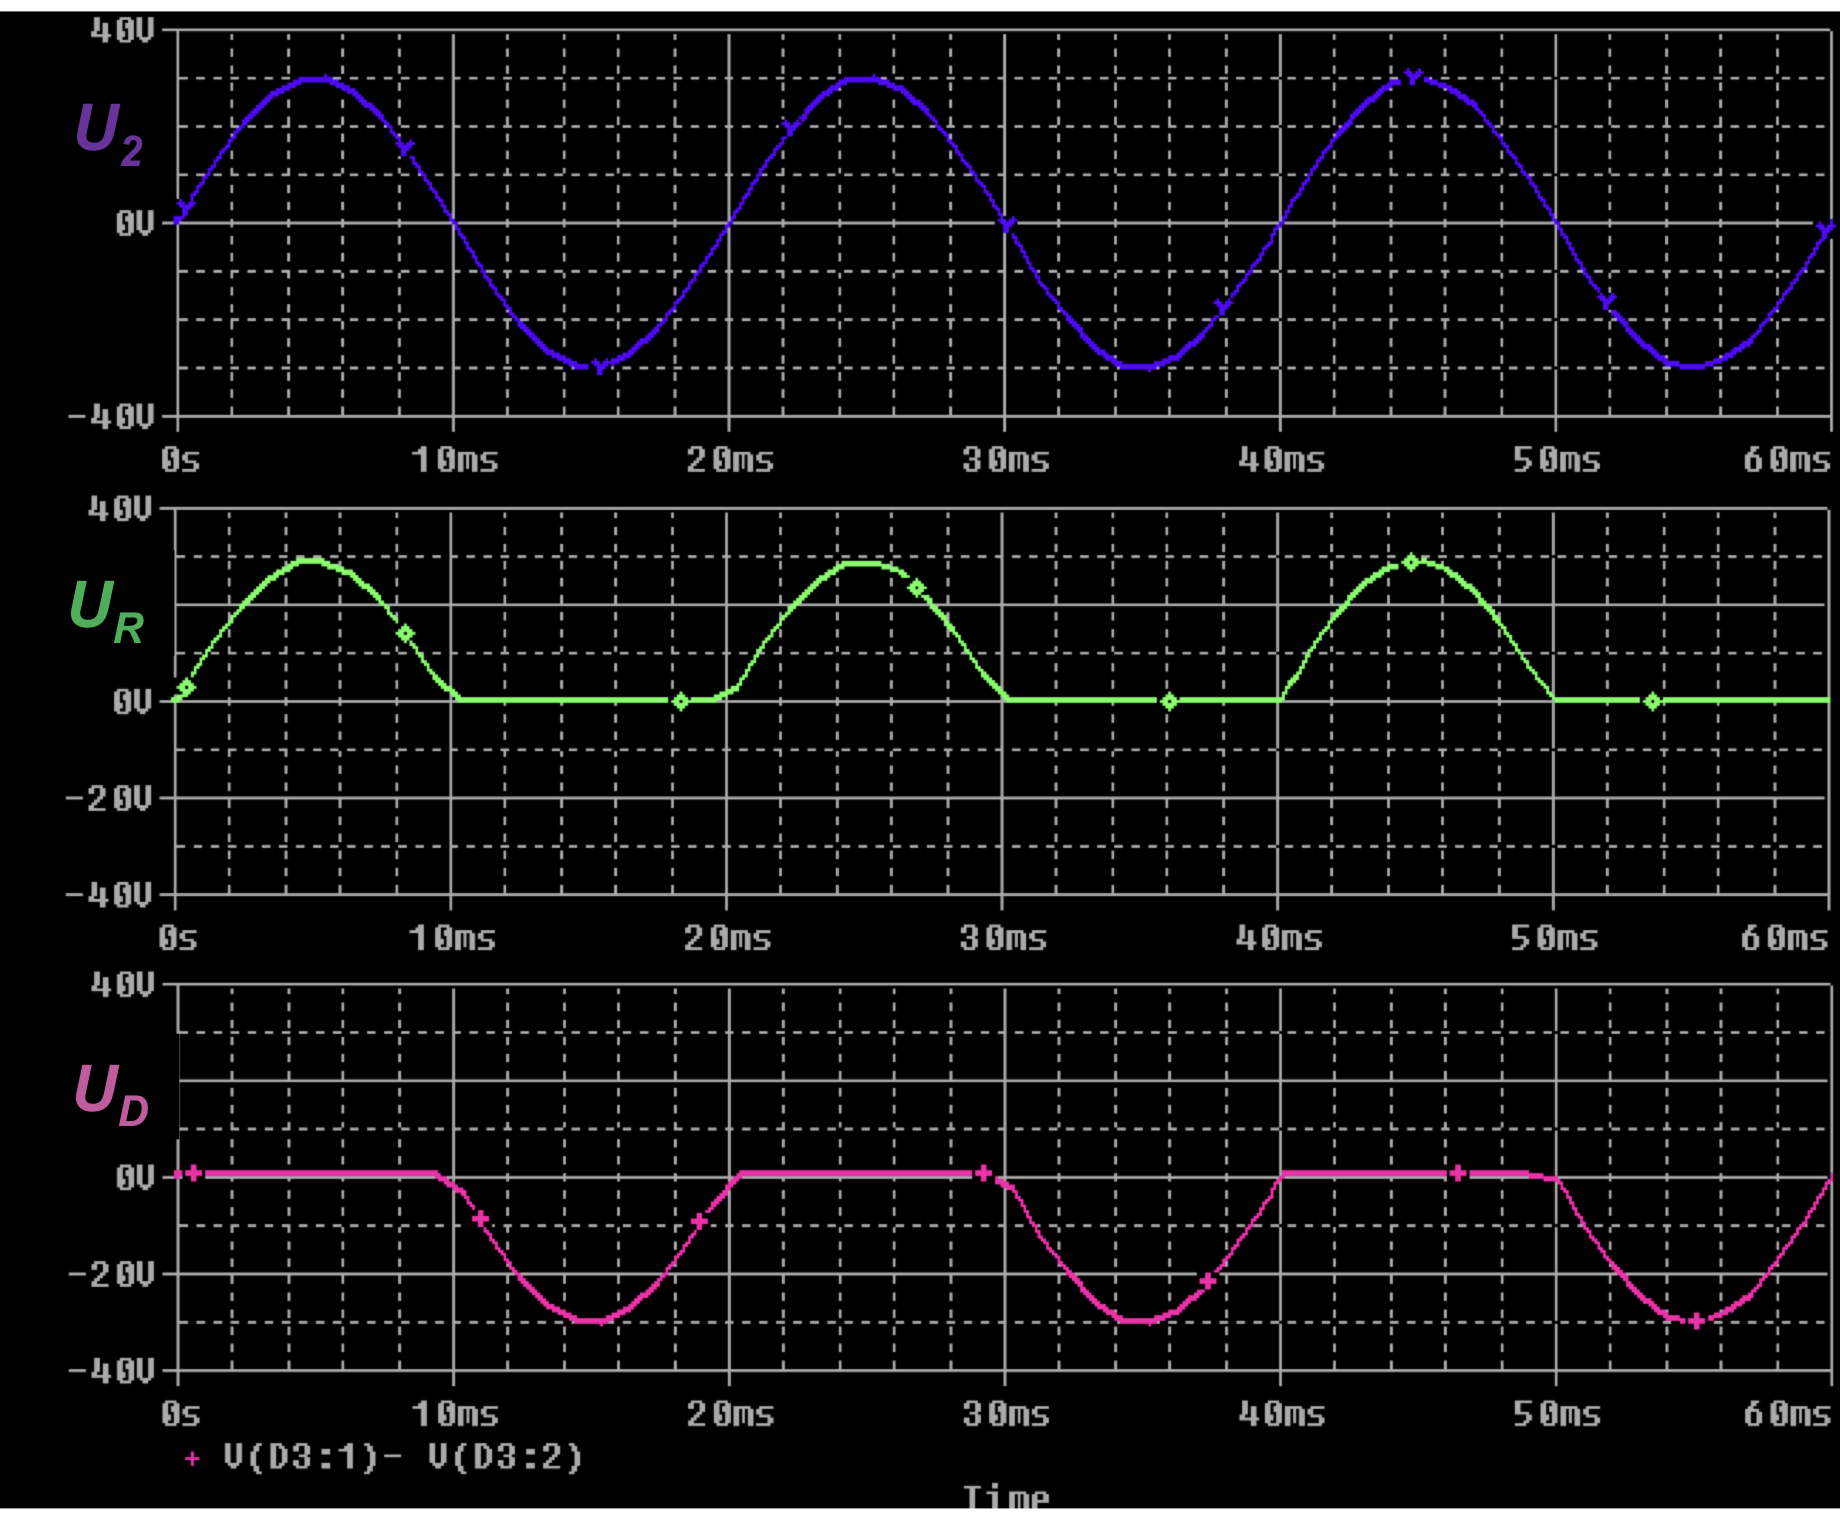
\includegraphics[width=0.85\linewidth]{images/M1U_verlauf.png}
\end{center}
\begin{center}
    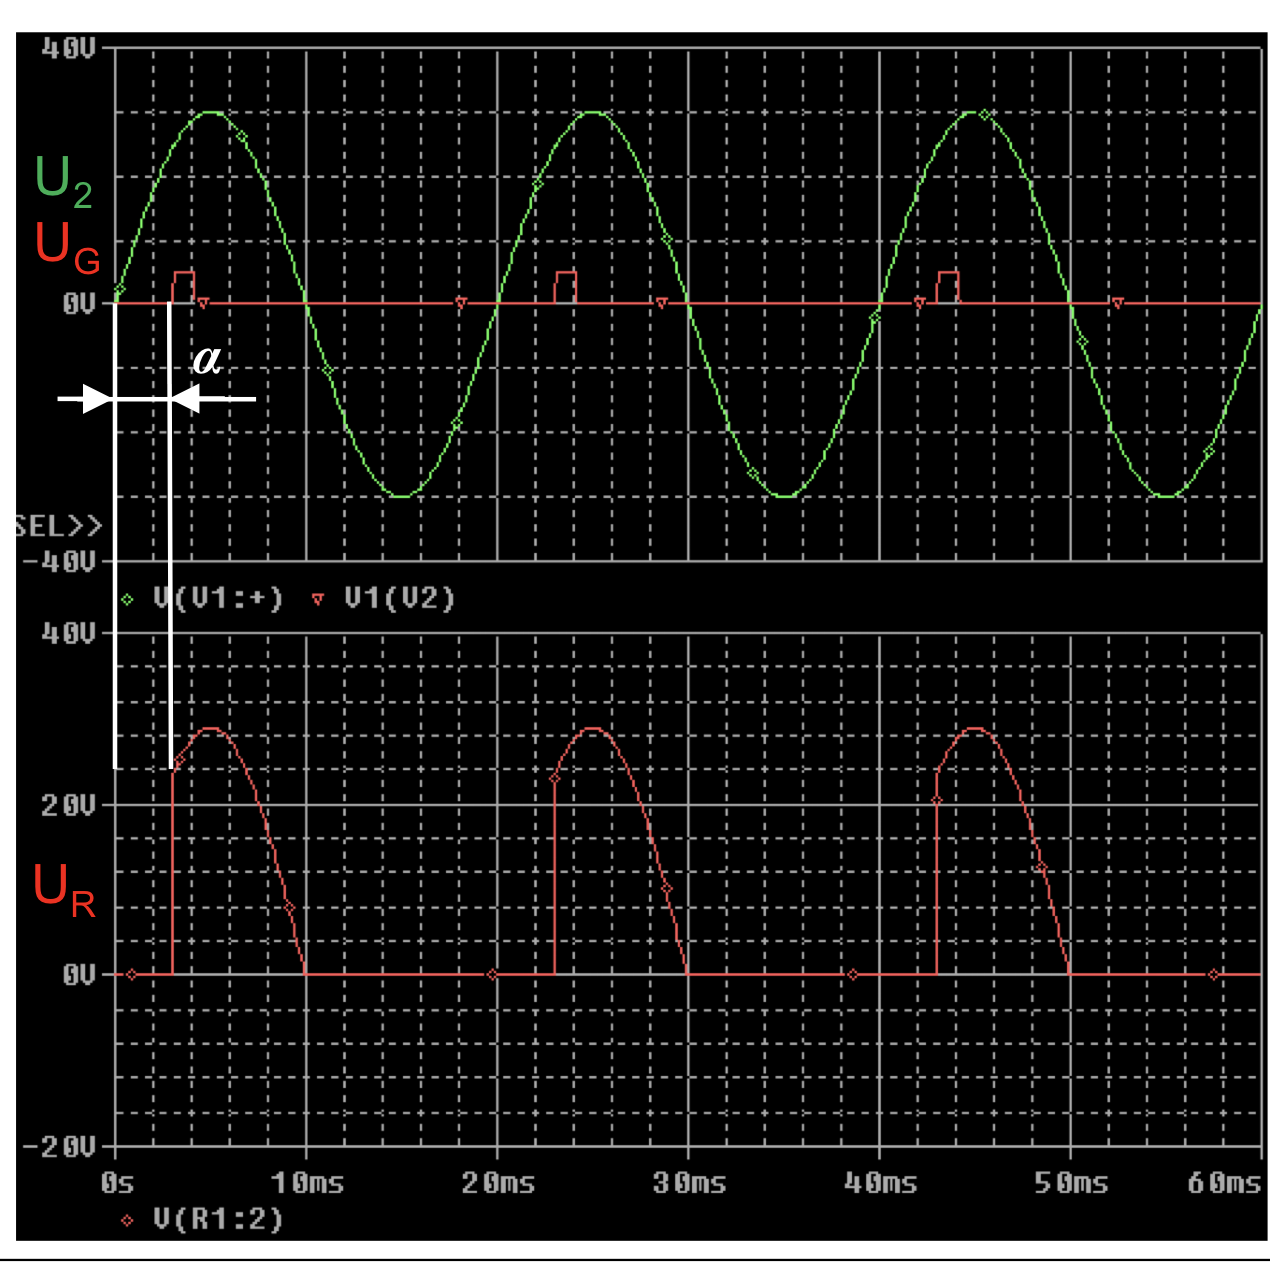
\includegraphics[width=0.85\linewidth]{images/M1C_Verlauf.png}
\end{center}

\textbf{Aussage:}
\begin{itemize}
    \item Negative Halbwelle wird abgeschnitten.
    \item Ausgang ist stark nichtsinusförmig.
\end{itemize}

\subsection{Mittelwert der Ausgangsspannung}

Definition:
\[
\cbl{\overline{u_2} = \frac{1}{T} \int_0^T u_2(t)\,\diff t.}
\]

Da $u_2(t)=0$ für $\pi<\omega t<2\pi$:
\[
\overline{u_2}
= \frac{1}{2\pi} \int_0^\pi \hat U \sin(\theta)\,\diff \theta
= \cbl{\frac{\hat U}{\pi}.}
\]

Interpretation:
\begin{itemize}
    \item Der Gleichwert ist proportional zur Scheitelspannung.
    \item Deutlich kleiner als der Mittelwert eines Vollweggleichrichters.
\end{itemize}

\subsection{Effektivwert der Ausgangsspannung}

Definition:
\[
\cbl{U_{2,\mathrm{RMS}} = \sqrt{\frac{1}{T} \int_0^T u_2^2(t)\,\diff t}.}
\]

\[
U_{2,\mathrm{RMS}}
= \sqrt{ \frac{1}{2\pi} \int_0^\pi \hat U^2 \sin^2(\theta)\,\diff \theta }
= \cbl{\frac{\hat U}{2}.}
\]

\subsection{Ohmsche Last ($R$-Last)}

\subsubsection{Stromverlauf}

\[
\cbl{i(t) = \frac{u_2(t)}{R}.}
\]

Eigenschaften:
\begin{itemize}
    \item Stromform identisch zur Spannung.
    \item Strom ist null während der negativen Halbwelle.
\end{itemize}

\subsubsection{Mittelwert des Stroms}

\[
\cbl{\overline{i} = \frac{\overline{u_2}}{R} = \frac{\hat U}{\pi R}.}
\]

\subsubsection{Effektivwert des Stroms}

\[
\cbl{I_{\mathrm{RMS}} = \frac{U_{2,\mathrm{RMS}}}{R} = \frac{\hat U}{2R}.}
\]

\subsubsection{Wirkleistung}

\[
\cbl{P = R \, I_{\mathrm{RMS}}^2 = \frac{\hat U^2}{4R}.}
\]

\subsection{Skizze 2: Strom bei ohmscher Last}

\begin{center}
\begin{tikzpicture}[scale=1]
\draw[->] (0,0) -- (8,0) node[right] {$t$};
\draw[->] (0,0) -- (0,3) node[above] {$i(t)$};

\draw (0,0) .. controls (1,2.5) .. (2,0);
\draw (4,0) .. controls (5,2.5) .. (6,0);

\draw[dashed] (0,1) -- (8,1) node[right] {$\overline{i}$};
\draw[dashed] (0,1.7) -- (8,1.7) node[right] {$I_{\mathrm{RMS}}$};

\draw (2,0) node[below] {$\pi/\omega$};
\draw (4,0) node[below] {$2\pi/\omega$};
\end{tikzpicture}
\end{center}

\subsection{Induktive Last ($R$-$L$-Last)}

\subsubsection{Grundgleichung}

Während Leitphase:
\[
\cbl{u_1(t) = R\,i(t) + L\,\frac{di(t)}{dt}.}
\]

Eigenschaften:
\begin{itemize}
    \item Strom ist \textbf{phasenverschoben}.
    \item Strom kann über $\pi$ hinaus weiterfliessen.
    \item Diode leitet länger als eine Halbwelle.
\end{itemize}

\crd{\textrightarrow\ Bei R-L-Last endet der Strom \textbf{nicht} exakt bei $\omega t=\pi$.}

\subsubsection{Stromform}

Qualitativ:
\begin{itemize}
    \item Strom steigt in der positiven Halbwelle.
    \item Strom fällt exponentiell in der Sperrphase.
    \item Es kann eine \textbf{Stromlücke} auftreten oder nicht.
\end{itemize}

\subsection{Skizze 3: Strom bei R-L-Last}

\begin{center}
\begin{tikzpicture}[scale=1]
\draw[->] (0,0) -- (8,0) node[right] {$t$};
\draw[->] (0,0) -- (0,3) node[above] {$i(t)$};

\draw (0,0) .. controls (1,2.2) .. (2,1.5)
      .. controls (3,1.0) .. (4,0.5)
      .. controls (5,0.2) .. (6,0);

\draw[dashed] (2,0) -- (2,-1) node[below] {$\pi/\omega$};

\draw (4,2.5) node[right] {Strom klingt ab};
\end{tikzpicture}
\end{center}

\textbf{Aussage:}
\begin{itemize}
    \item Induktivität glättet den Strom.
    \item Leitphase verlängert sich über $\pi$ hinaus.
\end{itemize}

\subsection{Typische Prüfungsresultate (Merksätze)}

\[
\overline{u_2} = \dfrac{\hat U}{\pi}
\]

\[
U_{2,\mathrm{RMS}} = \dfrac{\hat U}{2}
\]

\[
\overline{i} = \dfrac{\hat U}{\pi R}
\]

\[
I_{\mathrm{RMS}} = \dfrac{\hat U}{2R}
\]

\subsection{Typische Fehlerquellen}

\begin{itemize}
    \item Mittelwert und Effektivwert verwechselt.
    \item Integration über $2\pi$ statt nur über $\pi$.
    \item Stromform bei R-L-Last wie bei R-Last angenommen.
    \item Wirkungsleistung mit $\overline{u}\cdot\overline{i}$ berechnet.
\end{itemize}

\subsection{Minimal-Checkliste für Aufgaben}

\begin{enumerate}
    \item Leitintervall bestimmen ($0 \ldots \pi$ oder länger bei R-L).
    \item Mittelwert berechnen.
    \item Effektivwert berechnen.
    \item Strom über $i=u/R$ oder DGL bestimmen.
    \item Leistung über $P=R I_{\mathrm{RMS}}^2$ berechnen.
\end{enumerate}
%========================================================== 03M1U=========================================================================================================